\documentclass[11pt, a4paper]{article}
\usepackage[margin=1in]{geometry}
\usepackage{graphicx}
\usepackage{wrapfig}

\graphicspath{{images/}}

\title{Applied Machine Learning - Exploratory Sentiment Analysis}
\author{Poppy Z Grimes, Pinar Batat Buke, Zhifan Sun}
\date{November 2022}


\begin{document}
\maketitle 

\section{Task description}

Sentiment analysis is an important method within the sphere of natural language processing (NLP) to classify the positive or negative feeling within human text or speech. In the context of machine learning algorithms, sentiment analysis can be performed using both supervised and unsupervised methods. 

This project presents an exploratory analysis on the Stanford Sentiment Treebank (SST-5) dataset. We apply and build various task-based and feature-based algortihms and assess their performance in determining sentiment of online film reviews. We approach this by testing both full sentences and phrases. In addition, we explore how various pre-processing techniques effect our outcomes. This includes lemmetisation, human subjectivity etc.

Our primary aim is to build a model that can predict sentiment of sentences in the SST-5 dataset. To do this we will explore various algorithms and identify the one with the highest accuracy. Our work will compare outputs with previous work.
%compared with human based classifier?

Our secondary aim is to discuss the effect of data-preprocessing and formatting on the analysis. Methods incorporated include lemmetisation...


\section{Background and related work}
The SST-5 dataset is a repository of x film reviews from RottenTomatoes.com. The repository is organised into several files which split the data into sentences or phrases. Phrases from reviews have human-assigned sentiment scores where participants were asked to score on a continuous sliding scale seen in figure \ref{fig:sentiment_scale}.

\begin{wrapfigure}{l}{0.4\textwidth}
    \begin{center}
        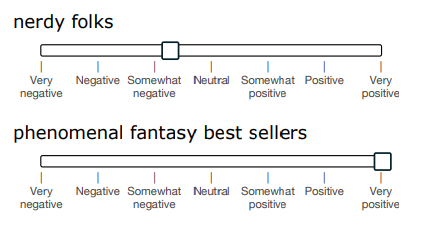
\includegraphics[width=0.38\textwidth]{sentiment_scale} 
    \end{center}
\caption{Continuous sentiment scale}
\label{fig:sentiment_scale}
\end{wrapfigure}

From this, phrases were assigned into one of five sentiment classes, producing a fine-grained sentiment labelled dataset. Unlike binary data, having five discrete classes overcomes the limitation of binary classifiers when faced with dual polarity (cite). A noteworthy example of this can be seen in negation \textit{e.g. 'this film hardly made me laugh'}. 

\subsection{Training on a recursive Neural Tensor Network (RNTN)}
This dataset was initially introduced by Socher \textit{et al.} (2013) to test a new neural network model with the aim to outperform previous algorithms on a) binary classification and b) fine-grained sentiment labels.

We also identified an analysis by Rao (2019) who took a similar approach to us in attempting to classify whole-sentences

\subsection{Bag of words (BOW)}
Bag of words is a popular method which tracks the polarity of individual words. It can be used to weight particularly positive or negative individual words accordingly. As a result, it is more successful in longer text strings. BOW exhibits weakness in that it does not account for grammatical, semantic or structural features within language. We decided to implement this as a baseline comparison but with the expectation of low performance.

\section{Task significance}

\section{Information on data pre-processing}

\subsection{Lemmetisation}

\subsection{Assigning sentiment scores to sentences}
The provided data set assigns sentiment scores only to individual phrases, or n-grams. For the purpose of our %supervised?
analysis, we need sentiment labels for full sentences. Of the multiple routes, we have chosen to explore two. Firstly, a manual human scoring of a sample of 100 sentences randomly chosen from the data. Second, we have pulled positive and negative words with high polarity with assigned sentiment from the labelled phrase-bank. For both routes, these will act as labels for training our classifiers. 

\section{Exploratory data analysis}

\section{Description of learning methods used}

\section{Results and evaluation}

\section{Conclusions}

\end{document}